\sloppy
\raggedbottom
\section{Prior public evaluations of Jev}
\label{app:prior}

Table~\ref{tab:prior} sets the public results next to ours. Every prior number in it was read from
its source on \PriorCheckedOn{} and is stored with the quoted text it came from; none was typed
into this paper. The protocols differ: each study uses its own template; the repository results
are for samples, with ECE over 10 bins; and the tabular benchmark uses a single
\PriorNStatsguysamWdbc-row split and a different serialization, which is the likely reason its
accuracy on Breast Cancer Wisconsin Diagnostic (\PriorAccStatsguysamWdbc) is far above ours
(\AccuracyJevWdbc).

\begin{table}[H]
  \caption{Prior public evaluations of zero-shot Jev on the datasets used here, next to our
    results at the default decision. Accuracy is at the argmax label.}
  \label{tab:prior}
  \centering\small
  \fittable{\begin{tabular}{llrrrrrr}
\toprule
 & & \multicolumn{3}{c}{Prior public evaluation} & \multicolumn{3}{c}{This paper (Jev, zero-shot)} \\
\cmidrule(lr){3-5}\cmidrule(lr){6-8}
Dataset & Source & $n$ & Acc. & ECE & $n$ & Acc. & ECE \\
\midrule
SST-2 & Deußer et al.~\citep{deusser2026jev} & 872 & 0.964 & 0.015 & 872 & 0.960 & 0.020 \\
AG News & Deußer et al.~\citep{deusser2026jev} & 7{,}600 & 0.885 & 0.077 & 7{,}600 & 0.879 & 0.082 \\
SST-2 & jevbench~\citep{jevbench2026} & 500 & 0.954 & 0.026 & 872 & 0.960 & 0.020 \\
AG News & jevbench~\citep{jevbench2026} & 500 & 0.843 & 0.112 & 7{,}600 & 0.879 & 0.082 \\
Breast Cancer Wisconsin Diagnostic & jev-classification-benchmark~\citep{statsguysam2026} & 114 & 0.842 & -- & 114 & 0.411 & 0.374 \\
German Credit & none found & -- & -- & -- & 200 & 0.467 & 0.364 \\
\bottomrule
\end{tabular}
}
\end{table}

\section{Protocol, label budgets and cost}
\label{app:protocol}

\paragraph{Models.}
Jev is queried through the \texttt{typesafe-sdk} Python client (version \SdkVersion) with one
\texttt{Choice} question per example; a missing tabular value is written as \texttt{unknown}, and
text is sent after collapsing whitespace. The text templates were tried once on
\TemplateCheckN{} training-split examples and frozen unchanged; the tabular templates were frozen
without being tried on data rows, because every row can be an evaluation row in some repeat.
XGBoost is trained with a fixed grid of \XgbGridSize{} configurations (tree depth and learning
rate), early stopping on the validation part (at most \XgbMaxRounds{} rounds, patience
\XgbPatience) and, for text, TF-IDF weights over unigrams and bigrams (at most \TfidfFeatures{}
features, \XgbTextBins{} histogram bins). BERT is \texttt{\BertModelId} (revision
\texttt{\BertRevision}); learning rates \BertLearningRates{} are each trained for up to
\BertMaxEpochs{} epochs (batch size \BertBatchSize) and the learning rate and epoch with the
lowest validation log-loss are kept, on the first split repeat for the tabular datasets. Inputs
are truncated at \BertMaxLengthGerman{} tokens (tabular), \BertMaxLengthAgnews{} (AG News) or
\BertMaxLengthSst{} (SST-2). Qwen is \texttt{\QwenModelId} (revision \texttt{\QwenRevision}) in
bf16. Its scores are computed with \texttt{transformers} \QwenTransformersVersion{} on
\texttt{\QwenScoringInstance}: the instruction and option list once per dataset, the rest of the
prompt once per item, and every option on a copy of that state, after a check on one item per
dataset that this equals a full recomputation. With thinking enabled the reasoning (greedy, at
most \ThinkMaxTokens{} tokens) is generated with vLLM~\citep{kwon2023vllm} \QwenVllmVersion{} and
the options are scored after it. All supervised training and all Qwen inference ran as managed
cloud training jobs (containers \texttt{sagemaker-xgboost:\XgbImageTag} and \breaktt{\BertImage}
for training).

\begin{table}[H]
  \caption{Labels used by each model, per split repeat. ``Early stopping, selection'' counts the
    validation labels used for early stopping and hyperparameter selection. Threshold selection
    applies to the binary datasets and reuses validation labels. The escalation threshold is
    selected on validation items predicted by both zero-shot models.}
  \label{tab:labels}
  \centering\small
  \fittable{\begin{tabular}{llrrrrr}
\toprule
Dataset & Model & Training & Early stopping, selection & Calibration & Threshold selection & Escalation threshold \\
\midrule
\multirow{4}{*}{German Credit} & Jev, zero-shot & 0 & 0 & 0 & 200 & 200 \\
 & Qwen3.6-27B, zero-shot & 0 & 0 & 0 & 200 & 200 \\
 & XGBoost, supervised & 600 & 200 & 0 & 200 & -- \\
 & BERT, supervised & 600 & 200 & 0 & 200 & -- \\
\addlinespace
\multirow{4}{*}{Breast Cancer Wisconsin} & Jev, zero-shot & 0 & 0 & 0 & 114 & 114 \\
 & Qwen3.6-27B, zero-shot & 0 & 0 & 0 & 114 & 114 \\
 & XGBoost, supervised & 341 & 114 & 0 & 114 & -- \\
 & BERT, supervised & 341 & 114 & 0 & 114 & -- \\
\addlinespace
\multirow{4}{*}{SST-2} & Jev, zero-shot & 0 & 0 & 0 & 500 & 500 \\
 & Qwen3.6-27B, zero-shot & 0 & 0 & 0 & 500 & 500 \\
 & XGBoost, supervised & 65{,}349 & 2{,}000 & 0 & 2{,}000 & -- \\
 & BERT, supervised & 65{,}349 & 2{,}000 & 0 & 2{,}000 & -- \\
\addlinespace
\multirow{4}{*}{AG News} & Jev, zero-shot & 0 & 0 & 0 & 0 & 500 \\
 & Qwen3.6-27B, zero-shot & 0 & 0 & 0 & 0 & 500 \\
 & XGBoost, supervised & 115{,}000 & 5{,}000 & 0 & 0 & -- \\
 & BERT, supervised & 115{,}000 & 5{,}000 & 0 & 0 & -- \\
\bottomrule
\end{tabular}
}
\end{table}

\paragraph{Budget and cost.}
The study was capped at \JevCap{} Jev inferences and used \JevInferencesUsed{}
(\JevRequestsPredict{} for predictions, \JevRequestsExplain{} for explanations,
\JevRequestsEscalationVal{} for escalation validation items, \JevRequestsTemplate{} for template
checks, \JevRequestsSmoke{} for connectivity checks). Every request is counted in a persistent
ledger before it is sent, and client retries are disabled; \JevFailedRequests{} requests failed.
Token counts exist for \JevRequestsWithTokens{} of the requests: \JevInputTokensM{} million input
tokens, USD~\JevCostUSD{} at USD~\JevPricePerMTok{} per million (Table~\ref{tab:cost}). All cloud
jobs together cost about USD~\AwsCostTotalUSD{} at list prices, under a limit of
USD~\AwsSpendLimit: USD~\AwsCostUSDXgb{} for XGBoost, USD~\AwsCostUSDBert{} for BERT
(\AwsGpuHoursBert{} GPU hours) and USD~\AwsCostUSDQwen{} for Qwen (\AwsGpuHoursQwen{} GPU hours),
counting stopped, failed and repeated executions. XGBoost was run a second time on every dataset
to record its inference time, and its predictions were \XgbRerunPredictions{} to the first ones.
Costs are computed from recorded token counts and from job records at list prices, not from
invoices.

\paragraph{A dataset that was run and removed.}
A fifth dataset, \RemovedDataset, was run and then removed from the study, because the
four-model comparison could not be completed on it within the compute limit. Everything spent on
it remains in the totals above: \RemovedJevRequests{} Jev requests (\RemovedJevTokensM{} million
input tokens, USD~\RemovedJevUSD), USD~\RemovedAwsDedicatedUSD{} of cloud jobs dedicated to it
(\RemovedAwsDedicatedExecutions{} executions), and a part of the USD~\RemovedAwsSharedUSD{} spent
on \RemovedAwsSharedExecutions{} exploratory Qwen executions that also covered other datasets and
cannot be split. No result for it is reported.

\paragraph{Societal impact.}
Two of the datasets stand for decisions that affect people: credit and medical diagnosis. Our
results are a caution for such uses. A zero-shot model's default decision was biased towards the
adverse class on both, on German Credit even with no evidence in the input, and nothing in its
text output would have revealed it. The positive side is that a class distribution makes the
bias measurable with standard tools and, where the ranking is sound, repairable with a small
labelled sample. The results describe four public benchmarks and one template per dataset and
should not be read as evidence that any of these models is fit or unfit for a deployment.

\paragraph{Uncertainty.}
For the held-out datasets we report 95\% bootstrap intervals (\BootstrapN{} resamples, fixed
seed). For the tabular datasets we report the mean and standard deviation over the \NRepeats{}
repeats; their test parts overlap across repeats, so the standard deviation describes split
variation, not an independent-sample standard error.

\begin{table}[H]
  \caption{Jev requests by stage. Input tokens are read from the logged responses and, for the
    \JevRequestsBeforeLoggingCached{} cached responses that predate the log, from the cache;
    \JevRequestsWithoutTokens{} request has no recorded token count. Output is not billed. The last
    row is the part of the total that was spent on the removed dataset.}
  \label{tab:cost}
  \centering\small
  \begin{tabular}{lrrrr}
\toprule
Stage & Requests & In request log & Input tokens (M) & Cost (USD) \\
\midrule
smoke & 3 & 2 & 0.00 & 0.000 \\
template & 60 & 60 & 0.06 & 0.003 \\
predict & 13{,}620 & 13{,}521 & 11.80 & 0.496 \\
explain & 35{,}317 & 35{,}317 & 25.81 & 1.084 \\
escalation\_val & 1{,}000 & 1{,}000 & 1.37 & 0.057 \\
\midrule
all stages & 50{,}000 & 49{,}900 & 39.04 & 1.640 \\
of which Banking77 (removed) & 9{,}198 & 9{,}198 & 21.10 & 0.886 \\
\bottomrule
\end{tabular}

\end{table}

\section{Full metrics and calibration}
\label{app:metrics}

\begin{table}[H]
  \caption{Classification metrics on identical evaluation examples. Brackets: 95\% bootstrap
    intervals (held-out datasets). $\pm$: standard deviation over \NRepeats{} split repeats
    (tabular datasets).}
  \label{tab:metrics}
  \centering\small
  \setlength{\tabcolsep}{4pt}
  \fittable{\begin{tabular}{llcccc}
\toprule
Dataset & Model & Accuracy & Macro-F1 & ROC-AUC & PR-AUC \\
\midrule
\multirow{4}{*}{German Credit} & Jev, zero-shot & 0.467\,{\scriptsize$\pm$0.019} & 0.467\,{\scriptsize$\pm$0.019} & 0.537\,{\scriptsize$\pm$0.030} & 0.316\,{\scriptsize$\pm$0.023} \\
 & Qwen3.6-27B, zero-shot & 0.544\,{\scriptsize$\pm$0.023} & 0.457\,{\scriptsize$\pm$0.025} & 0.496\,{\scriptsize$\pm$0.035} & 0.304\,{\scriptsize$\pm$0.028} \\
 & XGBoost, supervised & 0.741\,{\scriptsize$\pm$0.031} & 0.657\,{\scriptsize$\pm$0.041} & 0.768\,{\scriptsize$\pm$0.031} & 0.574\,{\scriptsize$\pm$0.046} \\
 & BERT, supervised & 0.705\,{\scriptsize$\pm$0.008} & 0.473\,{\scriptsize$\pm$0.083} & 0.683\,{\scriptsize$\pm$0.069} & 0.467\,{\scriptsize$\pm$0.071} \\
\addlinespace
\multirow{4}{*}{Breast Cancer Wisconsin} & Jev, zero-shot & 0.411\,{\scriptsize$\pm$0.014} & 0.343\,{\scriptsize$\pm$0.019} & 0.917\,{\scriptsize$\pm$0.021} & 0.878\,{\scriptsize$\pm$0.032} \\
 & Qwen3.6-27B, zero-shot & 0.825\,{\scriptsize$\pm$0.020} & 0.783\,{\scriptsize$\pm$0.029} & 0.969\,{\scriptsize$\pm$0.012} & 0.957\,{\scriptsize$\pm$0.012} \\
 & XGBoost, supervised & 0.949\,{\scriptsize$\pm$0.021} & 0.945\,{\scriptsize$\pm$0.023} & 0.985\,{\scriptsize$\pm$0.015} & 0.982\,{\scriptsize$\pm$0.015} \\
 & BERT, supervised & 0.778\,{\scriptsize$\pm$0.092} & 0.716\,{\scriptsize$\pm$0.182} & 0.853\,{\scriptsize$\pm$0.057} & 0.829\,{\scriptsize$\pm$0.044} \\
\addlinespace
\multirow{4}{*}{SST-2} & Jev, zero-shot & 0.960\,{\scriptsize[0.948,\,0.971]} & 0.960\,{\scriptsize[0.948,\,0.971]} & 0.987\,{\scriptsize[0.979,\,0.993]} & 0.986\,{\scriptsize[0.976,\,0.993]} \\
 & Qwen3.6-27B, zero-shot & 0.956\,{\scriptsize[0.943,\,0.968]} & 0.956\,{\scriptsize[0.943,\,0.968]} & 0.989\,{\scriptsize[0.984,\,0.994]} & 0.990\,{\scriptsize[0.984,\,0.995]} \\
 & XGBoost, supervised & 0.791\,{\scriptsize[0.763,\,0.819]} & 0.791\,{\scriptsize[0.762,\,0.818]} & 0.873\,{\scriptsize[0.848,\,0.896]} & 0.879\,{\scriptsize[0.849,\,0.905]} \\
 & BERT, supervised & 0.916\,{\scriptsize[0.896,\,0.935]} & 0.916\,{\scriptsize[0.896,\,0.935]} & 0.976\,{\scriptsize[0.968,\,0.983]} & 0.979\,{\scriptsize[0.971,\,0.986]} \\
\addlinespace
\multirow{4}{*}{AG News} & Jev, zero-shot & 0.879\,{\scriptsize[0.871,\,0.886]} & 0.878\,{\scriptsize[0.870,\,0.885]} & 0.961\,{\scriptsize[0.958,\,0.964]} & 0.901\,{\scriptsize[0.893,\,0.910]} \\
 & Qwen3.6-27B, zero-shot & 0.877\,{\scriptsize[0.870,\,0.885]} & 0.877\,{\scriptsize[0.870,\,0.884]} & 0.962\,{\scriptsize[0.958,\,0.965]} & 0.909\,{\scriptsize[0.900,\,0.917]} \\
 & XGBoost, supervised & 0.914\,{\scriptsize[0.908,\,0.921]} & 0.914\,{\scriptsize[0.908,\,0.921]} & 0.985\,{\scriptsize[0.983,\,0.986]} & 0.960\,{\scriptsize[0.955,\,0.965]} \\
 & BERT, supervised & 0.942\,{\scriptsize[0.936,\,0.947]} & 0.942\,{\scriptsize[0.937,\,0.947]} & 0.992\,{\scriptsize[0.991,\,0.993]} & 0.979\,{\scriptsize[0.976,\,0.982]} \\
\bottomrule
\end{tabular}
}
\end{table}

\begin{table}[H]
  \caption{Calibration: expected calibration error (\ECEBins{} equal-width bins), Brier score,
    log-loss, and mean confidence (mean of the maximum class probability). A reported probability
    of exactly zero for the true class is clipped at \LogLossClip{} in the log-loss.}
  \label{tab:calibration}
  \centering\small
  \setlength{\tabcolsep}{4pt}
  \fittable{\begin{tabular}{llcccc}
\toprule
Dataset & Model & ECE & Brier & Log-loss & Mean confidence \\
\midrule
\multirow{4}{*}{German Credit} & Jev, zero-shot & 0.364\,{\scriptsize$\pm$0.030} & 0.833\,{\scriptsize$\pm$0.041} & 2.136\,{\scriptsize$\pm$0.291} & 0.814 \\
 & Qwen3.6-27B, zero-shot & 0.136\,{\scriptsize$\pm$0.015} & 0.499\,{\scriptsize$\pm$0.017} & 0.694\,{\scriptsize$\pm$0.019} & 0.669 \\
 & XGBoost, supervised & 0.069\,{\scriptsize$\pm$0.017} & 0.346\,{\scriptsize$\pm$0.022} & 0.516\,{\scriptsize$\pm$0.027} & 0.757 \\
 & BERT, supervised & 0.060\,{\scriptsize$\pm$0.034} & 0.390\,{\scriptsize$\pm$0.024} & 0.574\,{\scriptsize$\pm$0.029} & 0.706 \\
\addlinespace
\multirow{4}{*}{Breast Cancer Wisconsin} & Jev, zero-shot & 0.374\,{\scriptsize$\pm$0.013} & 0.655\,{\scriptsize$\pm$0.014} & 0.865\,{\scriptsize$\pm$0.020} & 0.773 \\
 & Qwen3.6-27B, zero-shot & 0.072\,{\scriptsize$\pm$0.026} & 0.223\,{\scriptsize$\pm$0.012} & 0.341\,{\scriptsize$\pm$0.015} & 0.857 \\
 & XGBoost, supervised & 0.036\,{\scriptsize$\pm$0.010} & 0.074\,{\scriptsize$\pm$0.032} & 0.139\,{\scriptsize$\pm$0.064} & 0.966 \\
 & BERT, supervised & 0.115\,{\scriptsize$\pm$0.052} & 0.312\,{\scriptsize$\pm$0.062} & 0.486\,{\scriptsize$\pm$0.075} & 0.747 \\
\addlinespace
\multirow{4}{*}{SST-2} & Jev, zero-shot & 0.020\,{\scriptsize[0.014,\,0.034]} & 0.064\,{\scriptsize[0.047,\,0.082]} & 0.255\,{\scriptsize[0.138,\,0.397]} & 0.967 \\
 & Qwen3.6-27B, zero-shot & 0.023\,{\scriptsize[0.017,\,0.038]} & 0.073\,{\scriptsize[0.054,\,0.093]} & 0.159\,{\scriptsize[0.112,\,0.214]} & 0.974 \\
 & XGBoost, supervised & 0.026\,{\scriptsize[0.022,\,0.061]} & 0.290\,{\scriptsize[0.261,\,0.320]} & 0.451\,{\scriptsize[0.411,\,0.493]} & 0.799 \\
 & BERT, supervised & 0.054\,{\scriptsize[0.040,\,0.075]} & 0.138\,{\scriptsize[0.109,\,0.170]} & 0.259\,{\scriptsize[0.204,\,0.321]} & 0.966 \\
\addlinespace
\multirow{4}{*}{AG News} & Jev, zero-shot & 0.082\,{\scriptsize[0.076,\,0.090]} & 0.204\,{\scriptsize[0.192,\,0.216]} & 1.464\,{\scriptsize[1.337,\,1.591]} & 0.960 \\
 & Qwen3.6-27B, zero-shot & 0.099\,{\scriptsize[0.093,\,0.107]} & 0.219\,{\scriptsize[0.207,\,0.233]} & 0.925\,{\scriptsize[0.857,\,0.997]} & 0.976 \\
 & XGBoost, supervised & 0.032\,{\scriptsize[0.027,\,0.038]} & 0.135\,{\scriptsize[0.127,\,0.143]} & 0.270\,{\scriptsize[0.256,\,0.286]} & 0.887 \\
 & BERT, supervised & 0.018\,{\scriptsize[0.014,\,0.023]} & 0.091\,{\scriptsize[0.084,\,0.100]} & 0.179\,{\scriptsize[0.165,\,0.197]} & 0.958 \\
\bottomrule
\end{tabular}
}
\end{table}

\begin{figure}[H]
  \centering
  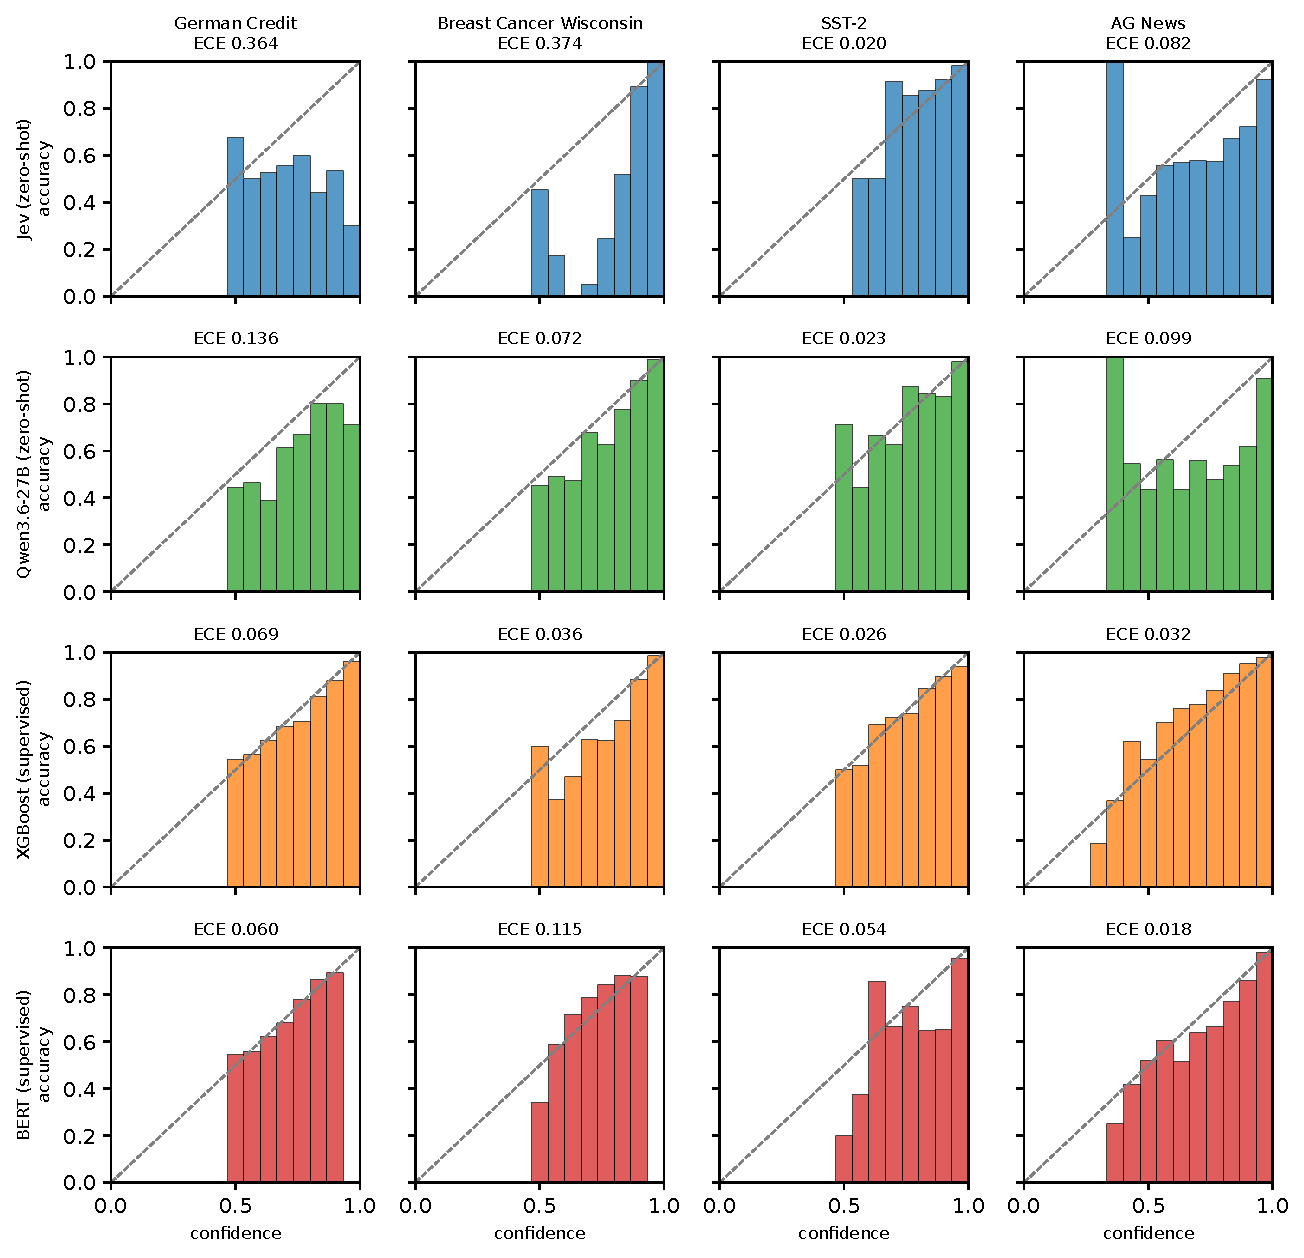
\includegraphics[width=\linewidth]{generated/figs/reliability}
  \caption{Reliability diagrams: accuracy against the maximum class probability, in \ECEBins{}
    equal-width bins. Rows, top to bottom: Jev and Qwen3.6-27B (zero-shot), XGBoost and BERT
    (supervised). Tabular datasets pool the test parts of all split repeats.}
  \label{fig:reliability}
\end{figure}

\section{Learning curves and thinking}
\label{app:learning}

On the text datasets, XGBoost sees only TF-IDF features and reaches 0.791 on SST-2 and 0.914 on AG News (zero-shot Jev: 0.960 and 0.879).
The learning curves (Figure~\ref{fig:learning}) put the comparison in terms of labels: on SST-2 it does not reach zero-shot Jev even with all 65{,}349 training labels; on AG News it first reaches zero-shot Jev at 28{,}752 training labels.


\begin{figure}[H]
  \centering
  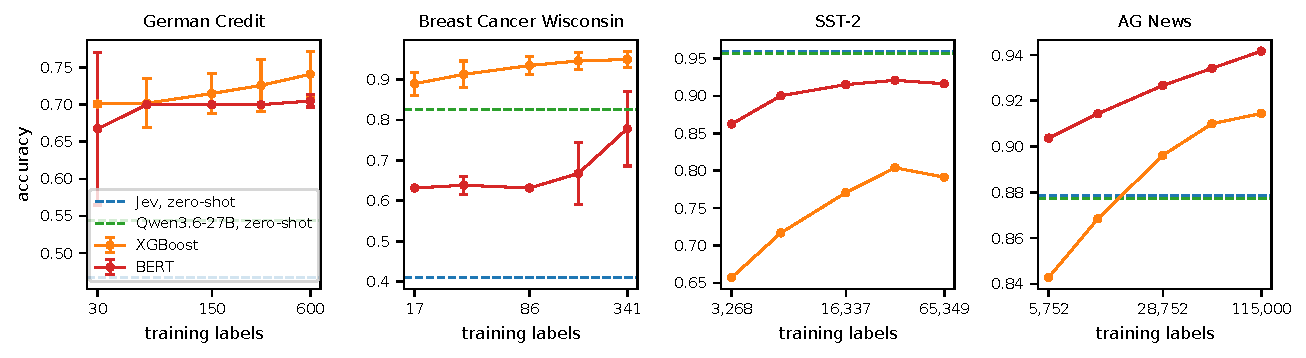
\includegraphics[width=\linewidth]{generated/figs/learning_curves}
  \caption{Accuracy of XGBoost and BERT on the evaluation examples against the number of
    training labels, with the zero-shot models as horizontal references.}
  \label{fig:learning}
\end{figure}

\begin{table}[H]
  \caption{XGBoost and BERT on the evaluation examples when trained on nested, stratified
    fractions of the training part with their selected configuration (mean over split repeats
    for the tabular datasets). The first row of each dataset gives the zero-shot models, at zero
    training labels, as accuracy / macro-F1.}
  \label{tab:learning}
  \centering\small
  \begin{tabular}{lrcccc}
\toprule
 & & \multicolumn{2}{c}{XGBoost, supervised} & \multicolumn{2}{c}{BERT, supervised} \\
\cmidrule(lr){3-4}\cmidrule(lr){5-6}
Dataset & Training labels & Accuracy & Macro-F1 & Accuracy & Macro-F1 \\
\midrule
\multirow{6}{*}{German Credit} & 0 & \multicolumn{4}{l}{Jev 0.467 / 0.467; Qwen3.6-27B 0.544 / 0.457} \\
 & 30 & 0.701 & 0.441 & 0.667 & 0.407 \\
 & 60 & 0.702 & 0.531 & 0.700 & 0.412 \\
 & 150 & 0.715 & 0.574 & 0.700 & 0.412 \\
 & 300 & 0.726 & 0.624 & 0.700 & 0.412 \\
 & 600 & 0.741 & 0.657 & 0.705 & 0.473 \\
\addlinespace
\multirow{6}{*}{Breast Cancer Wisconsin} & 0 & \multicolumn{4}{l}{Jev 0.411 / 0.343; Qwen3.6-27B 0.825 / 0.783} \\
 & 17 & 0.889 & 0.879 & 0.632 & 0.387 \\
 & 34 & 0.912 & 0.904 & 0.639 & 0.408 \\
 & 86 & 0.934 & 0.929 & 0.632 & 0.387 \\
 & 171 & 0.946 & 0.941 & 0.668 & 0.463 \\
 & 341 & 0.949 & 0.945 & 0.778 & 0.716 \\
\addlinespace
\multirow{6}{*}{SST-2} & 0 & \multicolumn{4}{l}{Jev 0.960 / 0.960; Qwen3.6-27B 0.956 / 0.956} \\
 & 3{,}268 & 0.657 & 0.654 & 0.862 & 0.861 \\
 & 6{,}535 & 0.717 & 0.713 & 0.900 & 0.900 \\
 & 16{,}337 & 0.771 & 0.769 & 0.915 & 0.915 \\
 & 32{,}674 & 0.804 & 0.804 & 0.921 & 0.921 \\
 & 65{,}349 & 0.791 & 0.791 & 0.916 & 0.916 \\
\addlinespace
\multirow{6}{*}{AG News} & 0 & \multicolumn{4}{l}{Jev 0.879 / 0.878; Qwen3.6-27B 0.877 / 0.877} \\
 & 5{,}752 & 0.843 & 0.842 & 0.904 & 0.904 \\
 & 11{,}500 & 0.868 & 0.868 & 0.914 & 0.914 \\
 & 28{,}752 & 0.896 & 0.896 & 0.927 & 0.927 \\
 & 57{,}500 & 0.910 & 0.910 & 0.934 & 0.934 \\
 & 115{,}000 & 0.914 & 0.914 & 0.942 & 0.942 \\
\bottomrule
\end{tabular}

\end{table}

\paragraph{Thinking.}
On the \ThinkSubsampleN{} items per dataset where Qwen also reasoned before answering, its
macro-F1 rose on every dataset: from \ThinkSubFOneQwenWdbc{} to \ThinkSubFOneQwenThinkWdbc{} on
Breast Cancer Wisconsin Diagnostic, \ThinkSubFOneQwenGerman{} to \ThinkSubFOneQwenThinkGerman{}
on German Credit, \ThinkSubFOneQwenSst{} to \ThinkSubFOneQwenThinkSst{} on SST-2 and
\ThinkSubFOneQwenAgnews{} to \ThinkSubFOneQwenThinkAgnews{} on AG News. These are small samples,
and the reasoning is long (\ThinkTokensWdbc{} tokens on average on Breast Cancer Wisconsin
Diagnostic, with \ThinkTruncatedGerman{} of German Credit items reaching the limit). Reasoning on
every item was projected at USD~\QwenThinkingAllProjectedUSD, which \QwenThinkingAllFits{} our
spending limit with a safety margin, so it was not run.

\begin{table}[H]
  \caption{Macro-F1 on the thinking subsample. Every model is scored on the same items.
    ``Thinking tokens'' is the mean length of the reasoning and ``Truncated'' the share of items
    whose reasoning reached the limit of \ThinkMaxTokens{} tokens.}
  \label{tab:thinking}
  \centering\small
  \fittable{\begin{tabular}{lrcccccrr}
\toprule
Dataset & $n$ & Jev & Qwen, off & Qwen, on & XGBoost & BERT & Thinking tokens & Truncated \\
\midrule
German Credit & 50 & 0.440 & 0.435 & 0.531 & 0.688 & 0.479 & 1{,}765 & 0.40 \\
Breast Cancer Wisconsin & 50 & 0.319 & 0.772 & 0.890 & 0.934 & 0.792 & 1{,}500 & 0.12 \\
SST-2 & 50 & 0.939 & 0.918 & 0.959 & 0.760 & 0.960 & 376 & 0.00 \\
AG News & 50 & 0.873 & 0.854 & 0.893 & 0.884 & 0.938 & 522 & 0.00 \\
\bottomrule
\end{tabular}
}
\end{table}

\section{Escalation: validation items}
\label{app:escalation}

The validation items for the escalation threshold are each repeat's validation part for the
tabular datasets, the \EscValLabelsSst{} threshold-selection items for SST-2, and
\EscValItemsNew{} seeded validation items for AG News that both models predicted for this
purpose.


\section{Threshold selection in full}
\label{app:thresholds}

Jev's threshold is selected on \ThrValLabelsJevGerman, \ThrValLabelsJevWdbc{} and
\ThrValLabelsJevSst{} validation labels for German Credit, Breast Cancer Wisconsin Diagnostic
and SST-2; on the tabular datasets this is repeated for each of the \NRepeats{} splits. On
Breast Cancer Wisconsin Diagnostic, at the default threshold Jev calls
\PredictedPositiveJevWdbc{} of the rows malignant, for a mean cost of
\ThrMeanCostDefaultJevWdbc; the analytic threshold (\ThresholdAnalyticJevWdbc) moves the wrong
way, to \ThrMeanCostAnalyticJevWdbc; the validation-selected threshold reaches
\ThrMeanCostValidationJevWdbc, with recall \ThrRecallValidationJevWdbc{} and precision
\ThrPrecisionValidationJevWdbc{} on malignant cases. On German Credit the cost is
\ThrMeanCostDefaultJevGerman{} at the default, \ThrMeanCostAnalyticJevGerman{} at the analytic and
\ThrMeanCostValidationJevGerman{} at the validation-selected threshold, and the lower cost is
bought by calling nearly every applicant bad (recall \ThrRecallValidationJevGerman, precision
\ThrPrecisionValidationJevGerman). On SST-2 the selected threshold
($t = \ThresholdValidationJevSst$) changes the cost only from \ThrMeanCostDefaultJevSst{} to
\ThrMeanCostValidationJevSst.


\begin{table}[H]
  \caption{Decisions at three thresholds on P(positive) for every model. Positive classes: bad
    (German Credit), malignant (Breast Cancer Wisconsin), positive (SST-2). Tabular values are
    means $\pm$ standard deviations over \NRepeats{} split repeats, and $t$ is the mean
    threshold. Costs: \CostRatioGerman{} (canonical), \CostRatioWdbc{} (illustrative),
    \CostRatioSst{} (illustrative).}
  \label{tab:thresholds-all}
  \centering\scriptsize
  \setlength{\tabcolsep}{3.5pt}
  \fittable{\begin{tabular}{lllcccccc}
\toprule
Dataset & Model & Threshold & $t$ & Precision & Recall & F1 (pos.) & Accuracy & Mean cost \\
\midrule
\multirow{12}{*}{German Credit} & \multirow{3}{*}{Jev, zero-shot} & default & 0.50 & 0.334\,{\scriptsize$\pm$0.012} & 0.790\,{\scriptsize$\pm$0.030} & 0.470\,{\scriptsize$\pm$0.016} & 0.465\,{\scriptsize$\pm$0.020} & 0.787\,{\scriptsize$\pm$0.048} \\
 &  & analytic & 0.17 & 0.313\,{\scriptsize$\pm$0.007} & 0.968\,{\scriptsize$\pm$0.018} & 0.473\,{\scriptsize$\pm$0.010} & 0.351\,{\scriptsize$\pm$0.016} & 0.686\,{\scriptsize$\pm$0.034} \\
 &  & validation-selected & 0.17 & 0.311\,{\scriptsize$\pm$0.008} & 0.960\,{\scriptsize$\pm$0.027} & 0.470\,{\scriptsize$\pm$0.011} & 0.350\,{\scriptsize$\pm$0.017} & 0.698\,{\scriptsize$\pm$0.042} \\
\cmidrule(lr){2-9}
 & \multirow{3}{*}{Qwen3.6-27B, zero-shot} & default & 0.50 & 0.244\,{\scriptsize$\pm$0.037} & 0.252\,{\scriptsize$\pm$0.043} & 0.248\,{\scriptsize$\pm$0.039} & 0.542\,{\scriptsize$\pm$0.023} & 1.356\,{\scriptsize$\pm$0.068} \\
 &  & analytic & 0.17 & 0.314\,{\scriptsize$\pm$0.009} & 0.955\,{\scriptsize$\pm$0.026} & 0.472\,{\scriptsize$\pm$0.012} & 0.360\,{\scriptsize$\pm$0.020} & 0.694\,{\scriptsize$\pm$0.043} \\
 &  & validation-selected & 0.14 & 0.306\,{\scriptsize$\pm$0.008} & 0.960\,{\scriptsize$\pm$0.039} & 0.464\,{\scriptsize$\pm$0.012} & 0.335\,{\scriptsize$\pm$0.024} & 0.713\,{\scriptsize$\pm$0.046} \\
\cmidrule(lr){2-9}
 & \multirow{3}{*}{XGBoost, supervised} & default & 0.50 & 0.604\,{\scriptsize$\pm$0.084} & 0.413\,{\scriptsize$\pm$0.071} & 0.488\,{\scriptsize$\pm$0.064} & 0.741\,{\scriptsize$\pm$0.031} & 0.963\,{\scriptsize$\pm$0.106} \\
 &  & analytic & 0.17 & 0.419\,{\scriptsize$\pm$0.017} & 0.883\,{\scriptsize$\pm$0.047} & 0.568\,{\scriptsize$\pm$0.021} & 0.597\,{\scriptsize$\pm$0.026} & 0.544\,{\scriptsize$\pm$0.062} \\
 &  & validation-selected & 0.17 & 0.415\,{\scriptsize$\pm$0.031} & 0.872\,{\scriptsize$\pm$0.091} & 0.560\,{\scriptsize$\pm$0.031} & 0.588\,{\scriptsize$\pm$0.057} & 0.566\,{\scriptsize$\pm$0.096} \\
\cmidrule(lr){2-9}
 & \multirow{3}{*}{BERT, supervised} & default & 0.50 & 0.231\,{\scriptsize$\pm$0.306} & 0.093\,{\scriptsize$\pm$0.137} & 0.125\,{\scriptsize$\pm$0.173} & 0.704\,{\scriptsize$\pm$0.007} & 1.384\,{\scriptsize$\pm$0.167} \\
 &  & analytic & 0.17 & 0.345\,{\scriptsize$\pm$0.051} & 0.930\,{\scriptsize$\pm$0.093} & 0.498\,{\scriptsize$\pm$0.038} & 0.426\,{\scriptsize$\pm$0.133} & 0.658\,{\scriptsize$\pm$0.048} \\
 &  & validation-selected & 0.21 & 0.352\,{\scriptsize$\pm$0.034} & 0.918\,{\scriptsize$\pm$0.085} & 0.506\,{\scriptsize$\pm$0.026} & 0.459\,{\scriptsize$\pm$0.085} & 0.639\,{\scriptsize$\pm$0.062} \\
\midrule
\multirow{12}{*}{Breast Cancer Wisconsin} & \multirow{3}{*}{Jev, zero-shot} & default & 0.50 & 0.382\,{\scriptsize$\pm$0.007} & 0.993\,{\scriptsize$\pm$0.012} & 0.552\,{\scriptsize$\pm$0.008} & 0.405\,{\scriptsize$\pm$0.014} & 0.605\,{\scriptsize$\pm$0.030} \\
 &  & analytic & 0.17 & 0.369\,{\scriptsize$\pm$0.001} & 1.000\,{\scriptsize$\pm$0.000} & 0.539\,{\scriptsize$\pm$0.001} & 0.370\,{\scriptsize$\pm$0.004} & 0.630\,{\scriptsize$\pm$0.004} \\
 &  & validation-selected & 0.77 & 0.605\,{\scriptsize$\pm$0.079} & 0.912\,{\scriptsize$\pm$0.083} & 0.721\,{\scriptsize$\pm$0.040} & 0.735\,{\scriptsize$\pm$0.068} & 0.395\,{\scriptsize$\pm$0.089} \\
\cmidrule(lr){2-9}
 & \multirow{3}{*}{Qwen3.6-27B, zero-shot} & default & 0.50 & 0.991\,{\scriptsize$\pm$0.019} & 0.531\,{\scriptsize$\pm$0.056} & 0.690\,{\scriptsize$\pm$0.048} & 0.825\,{\scriptsize$\pm$0.021} & 0.866\,{\scriptsize$\pm$0.104} \\
 &  & analytic & 0.17 & 0.838\,{\scriptsize$\pm$0.031} & 0.905\,{\scriptsize$\pm$0.032} & 0.870\,{\scriptsize$\pm$0.023} & 0.900\,{\scriptsize$\pm$0.018} & 0.240\,{\scriptsize$\pm$0.059} \\
 &  & validation-selected & 0.15 & 0.789\,{\scriptsize$\pm$0.058} & 0.926\,{\scriptsize$\pm$0.046} & 0.850\,{\scriptsize$\pm$0.027} & 0.878\,{\scriptsize$\pm$0.029} & 0.231\,{\scriptsize$\pm$0.059} \\
\cmidrule(lr){2-9}
 & \multirow{3}{*}{XGBoost, supervised} & default & 0.50 & 0.942\,{\scriptsize$\pm$0.023} & 0.919\,{\scriptsize$\pm$0.047} & 0.930\,{\scriptsize$\pm$0.030} & 0.949\,{\scriptsize$\pm$0.021} & 0.170\,{\scriptsize$\pm$0.088} \\
 &  & analytic & 0.17 & 0.879\,{\scriptsize$\pm$0.036} & 0.960\,{\scriptsize$\pm$0.046} & 0.917\,{\scriptsize$\pm$0.029} & 0.936\,{\scriptsize$\pm$0.022} & 0.124\,{\scriptsize$\pm$0.084} \\
 &  & validation-selected & 0.27 & 0.895\,{\scriptsize$\pm$0.042} & 0.943\,{\scriptsize$\pm$0.053} & 0.917\,{\scriptsize$\pm$0.026} & 0.937\,{\scriptsize$\pm$0.019} & 0.147\,{\scriptsize$\pm$0.089} \\
\cmidrule(lr){2-9}
 & \multirow{3}{*}{BERT, supervised} & default & 0.50 & 0.613\,{\scriptsize$\pm$0.333} & 0.593\,{\scriptsize$\pm$0.334} & 0.595\,{\scriptsize$\pm$0.321} & 0.778\,{\scriptsize$\pm$0.092} & 0.822\,{\scriptsize$\pm$0.574} \\
 &  & analytic & 0.17 & 0.560\,{\scriptsize$\pm$0.127} & 0.879\,{\scriptsize$\pm$0.080} & 0.671\,{\scriptsize$\pm$0.089} & 0.661\,{\scriptsize$\pm$0.161} & 0.518\,{\scriptsize$\pm$0.127} \\
 &  & validation-selected & 0.20 & 0.587\,{\scriptsize$\pm$0.103} & 0.845\,{\scriptsize$\pm$0.079} & 0.687\,{\scriptsize$\pm$0.079} & 0.709\,{\scriptsize$\pm$0.099} & 0.519\,{\scriptsize$\pm$0.168} \\
\midrule
\multirow{12}{*}{SST-2} & \multirow{3}{*}{Jev, zero-shot} & default & 0.50 & 0.979 & 0.941 & 0.960 & 0.960 & 0.040 \\
 &  & analytic & 0.50 & 0.979 & 0.941 & 0.960 & 0.960 & 0.040 \\
 &  & validation-selected & 0.36 & 0.975 & 0.959 & 0.967 & 0.967 & 0.033 \\
\cmidrule(lr){2-9}
 & \multirow{3}{*}{Qwen3.6-27B, zero-shot} & default & 0.50 & 0.981 & 0.932 & 0.956 & 0.956 & 0.044 \\
 &  & analytic & 0.50 & 0.981 & 0.932 & 0.956 & 0.956 & 0.044 \\
 &  & validation-selected & 0.29 & 0.972 & 0.953 & 0.962 & 0.962 & 0.038 \\
\cmidrule(lr){2-9}
 & \multirow{3}{*}{XGBoost, supervised} & default & 0.50 & 0.781 & 0.820 & 0.800 & 0.791 & 0.209 \\
 &  & analytic & 0.50 & 0.781 & 0.820 & 0.800 & 0.791 & 0.209 \\
 &  & validation-selected & 0.55 & 0.798 & 0.800 & 0.799 & 0.795 & 0.205 \\
\cmidrule(lr){2-9}
 & \multirow{3}{*}{BERT, supervised} & default & 0.50 & 0.901 & 0.939 & 0.920 & 0.916 & 0.084 \\
 &  & analytic & 0.50 & 0.901 & 0.939 & 0.920 & 0.916 & 0.084 \\
 &  & validation-selected & 0.49 & 0.901 & 0.939 & 0.920 & 0.916 & 0.084 \\
\bottomrule
\end{tabular}
}
\end{table}

\begin{figure}[H]
  \centering
  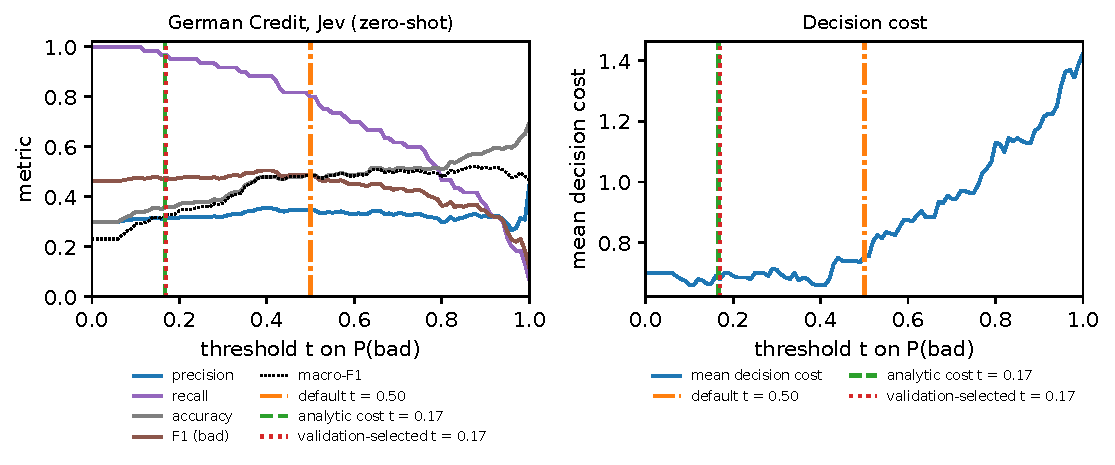
\includegraphics[width=0.8\linewidth]{generated/figs/threshold_german_jev}\\
  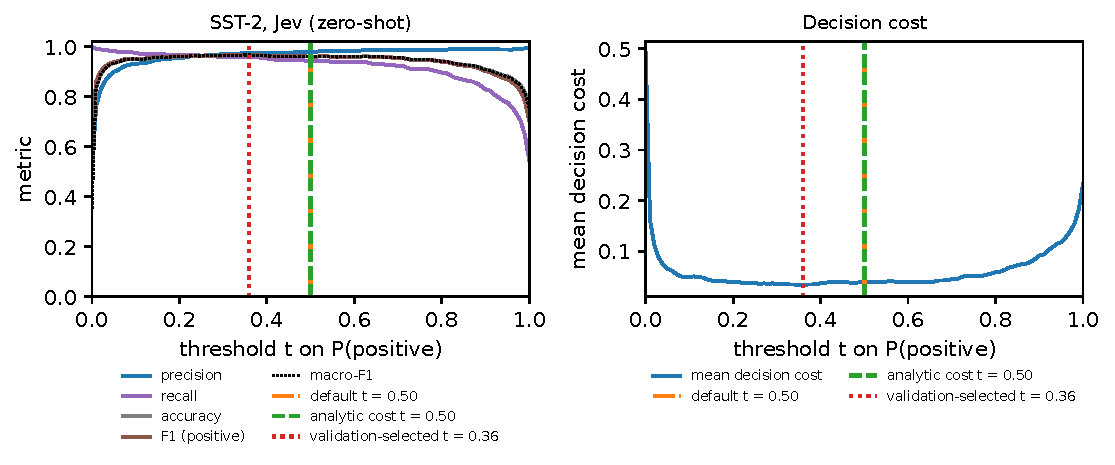
\includegraphics[width=0.8\linewidth]{generated/figs/threshold_sst2_jev}\\
  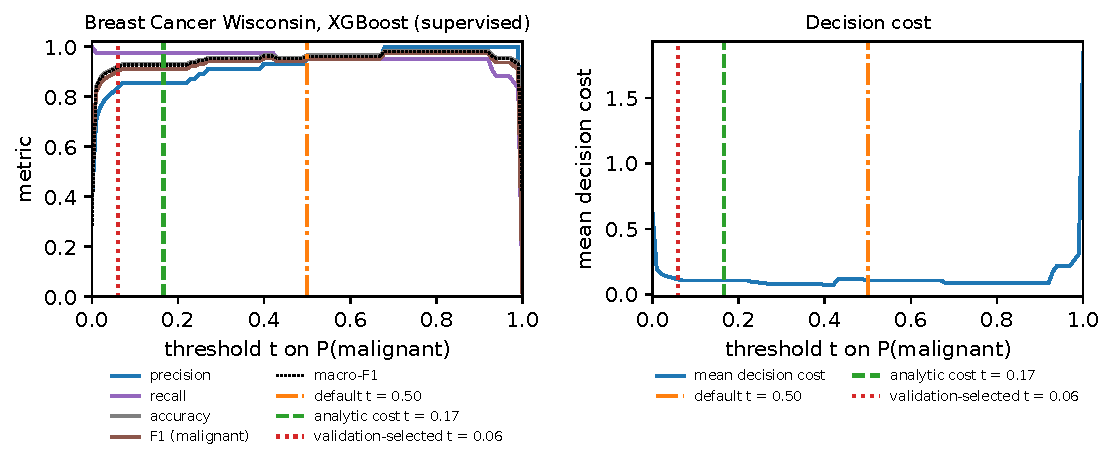
\includegraphics[width=0.8\linewidth]{generated/figs/threshold_wdbc_xgb}
  \caption{Threshold sweeps (first split repeat) for Jev on German Credit and SST-2, and for
    XGBoost on Breast Cancer Wisconsin Diagnostic. For SST-2 the costs are symmetric, so the
    analytic threshold coincides with the default.}
  \label{fig:threshold-more}
\end{figure}

\section{Importance sampling in full}
\label{app:importance}

For each dataset the pool is the fixed set of examples with cached Jev predictions. The sampling
procedure sees only those predictions: it draws $n$ items with replacement and asks for the
labels of the drawn items only. The Hansen--Hurwitz estimate of the error rate is
$\frac{1}{n}\sum_{j} \ell_{i_j}/(N q_{i_j})$, which is unbiased for any positive $q$, and accuracy
is one minus it. We run \ISTrials{} seeded trials at each budget $n \in \{\ISBudgets\}$ and
compare with the full-pool accuracy, which is used only as ground truth.


\begin{figure}[H]
  \centering
  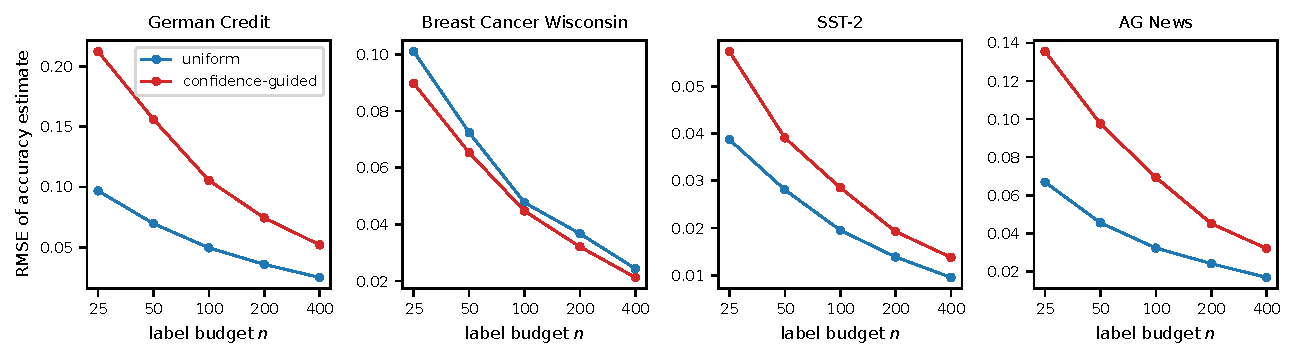
\includegraphics[width=\linewidth]{generated/figs/importance}
  \caption{RMSE of the accuracy estimate against the label budget.}
  \label{fig:is}
\end{figure}

Two things explain the result. First, because of the rounding, a large part of each text pool has
a reported uncertainty of exactly zero: \IsZeroUncertaintySst{} of \IsPoolSst{} items on SST-2
and \IsZeroUncertaintyAgnews{} of \IsPoolAgnews{} on AG News. Those items receive only the minimum
sampling probability $\varepsilon/N$, yet they contain \IsErrorsZeroUncertaintySst{} of the
\IsErrorsSst{} errors on SST-2 and \IsErrorsZeroUncertaintyAgnews{} of \IsErrorsAgnews{} on AG
News. Second, for a 0/1 loss a proposal proportional to the expected loss has the same variance
as uniform sampling under perfect calibration, and the optimum is proportional to the square
root of the expected loss. With $\alpha = \ISAlphaSqrt$ the ratios at $n = \ISMaxBudget$ are
\IsVarRatioHalfWdbc{} on Breast Cancer Wisconsin Diagnostic, \IsVarRatioHalfGerman{} on German
Credit, \IsVarRatioHalfSst{} on SST-2 and \IsVarRatioHalfAgnews{} on AG News: still below 1 on
\IsDatasetsSqrtBelowOne{} of the \NDatasets. Here the check says to sample uniformly unless the
reported uncertainties are first floored or recalibrated.

\section{Explanations in full}
\label{app:explain}

KernelSHAP uses \ShapCoalitions{} coalitions with the all-removed input as background, and LIME
\LimeSamples{} samples. Text examples were drawn among those with \ExMinWords{} to \ExMaxWords{}
words (\ExEligibleSst{} of \NTestSst{} for SST-2, \ExEligibleAgnews{} of \NTestAgnews{} for AG
News), so that deleting five words is meaningful. Faithfulness is tested by deleting the top-$k$
attributed units and re-querying Jev, against deleting $k$ random units (\ExRandomDraws{} draws).
KernelSHAP's attributions plus its base value reconstruct Jev's probability exactly (largest
additivity error \ExAdditivityMax). The two methods agree moderately to well on German Credit
and SST-2 ($\tau = \ExTauGerman$ and \ExTauSst) and little on Breast Cancer Wisconsin Diagnostic
and AG News ($\tau = \ExTauWdbc$ and \ExTauAgnews), where LIME's linear surrogate fits poorly
($R^2 = \ExLimeRTwoWdbc$ and \ExLimeRTwoAgnews, against \ExLimeRTwoGerman{} on German Credit).
With every feature removed, Jev assigns the positive class a probability of
\ExEmptyInputPositiveGerman{} on German Credit and \ExEmptyInputPositiveWdbc{} on Breast Cancer
Wisconsin Diagnostic, where the true shares are \TruePositiveGerman{} and \TruePositiveWdbc.
Perturbation methods are paid for in model calls: at most \ExRequestsPerExample{} per example
here, and \ExRequestsTotal{} requests in total (USD~\ExCostUSD), between \ExRequestsMin{} and
\ExRequestsMax{} per dataset after caching repeated inputs.


\begin{figure}[H]
  \centering
  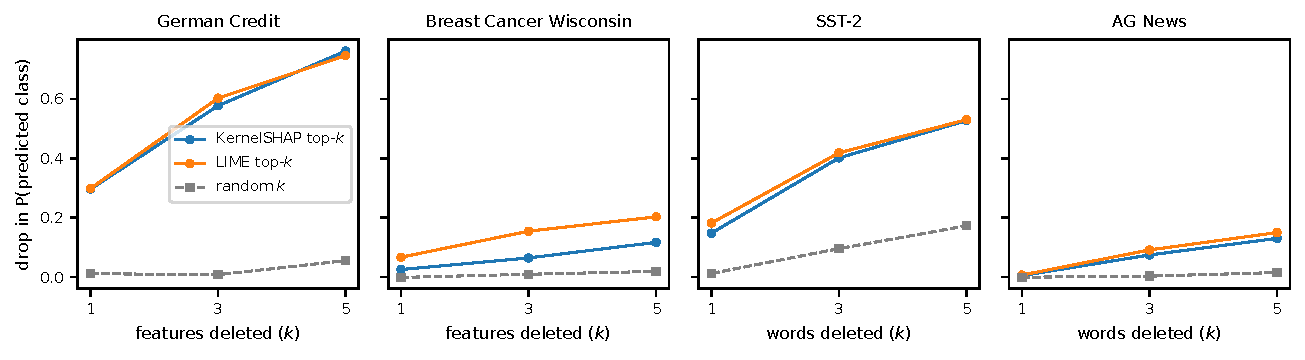
\includegraphics[width=\linewidth]{generated/figs/faithfulness}
  \caption{Deletion test: mean drop in Jev's predicted-class probability after deleting the $k$
    top-attributed units (KernelSHAP, LIME) or $k$ random units.}
  \label{fig:faithfulness}
\end{figure}

\begin{figure}[H]
  \centering
  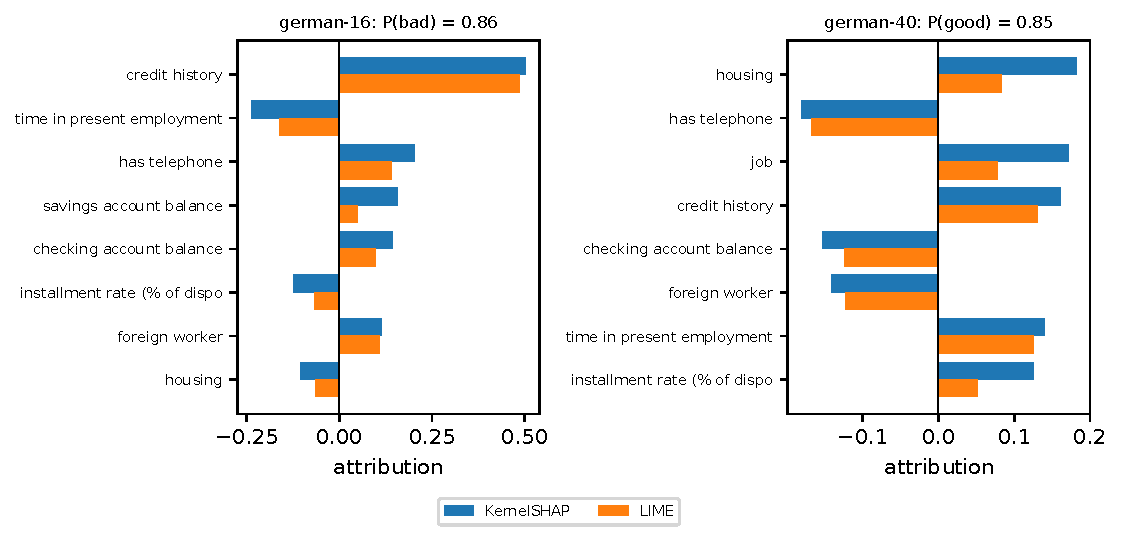
\includegraphics[width=0.49\linewidth]{generated/figs/attributions_german}\hfill
  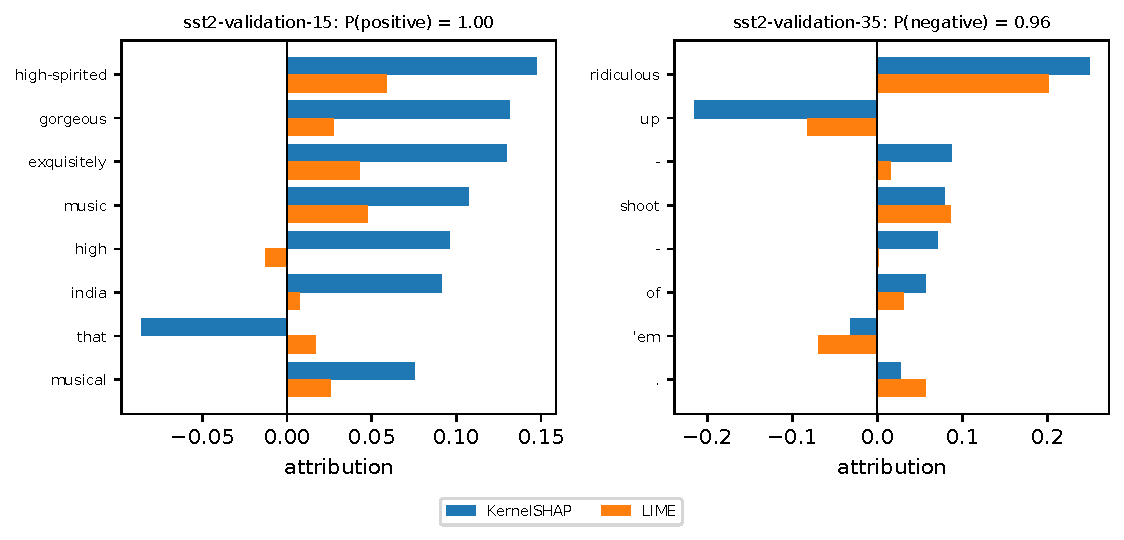
\includegraphics[width=0.49\linewidth]{generated/figs/attributions_sst2}
  \caption{KernelSHAP and LIME attributions for two German Credit applicants (left) and two
    SST-2 sentences (right): the eight units with the largest absolute KernelSHAP value.}
  \label{fig:attributions}
\end{figure}

\section{Exact requests and responses}
\label{app:payloads}

One complete exchange per dataset, copied from the request log. The example is the first
evaluation example, in a seeded order, whose request is in the log. The request and response
bodies are the JSON that crossed the wire, re-indented for reading; non-ASCII characters are shown
as JSON escapes. Headers are not recorded, so the API key cannot appear.

The \AuditUnlogged{} requests made before the log existed are not shown, because there is nothing
to copy. For \AuditUnloggedCached{} of them the response was cached in parsed form; regenerating
their requests from code and hashing them reproduces \AuditRegeneratedMatches{} of the
\AuditUnloggedCached{} stored cache keys, which shows that the same input, instructions, label
descriptions and model version were sent, but does not recover the payloads or the raw responses.
The remaining one was a connectivity check that was not cached.

\subsection*{German Credit}
Example \texttt{german-870}, gold label \texttt{good}; ledger number 951, sent 2026-09-30T13:\allowbreak{}43:\allowbreak{}22.039+00:\allowbreak{}00; \texttt{POST https://api.typesafe.ai/\allowbreak{}v1/\allowbreak{}systemone}; SDK \texttt{typesafe-sdk 0.7.2}; requested model \texttt{jev-1.13.0}, reported model \texttt{jev-1.13.0}; HTTP status 200; latency 0.18\,s.

\noindent\textbf{Request body as sent}
\begin{lstlisting}
{
 "state": "checking account balance: no checking account\nloan duration (months): 36\ncredit history: delayed previously\nloan purpose: furniture/equipment\ncredit amount (DM): 7678\nsavings account balance: 500 to 1000 DM\ntime in present employment: 4 to 7 years\ninstallment rate (% of disposable income): 2\npersonal status and sex: female div/dep/mar\nother debtors / guarantors: none\nyears at present residence: 4\nmost valuable property: car\nage (years): 40\nother installment plans: none\nhousing: own\nnumber of existing credits at this bank: 2\njob: skilled\nnumber of dependents: 1\nhas telephone: yes\nforeign worker: yes",
 "model": "jev-1.13.0",
 "questions": {
  "label": {
   "type": "choice",
   "instructions": "Assess the credit risk of a bank loan applicant described below. Fields that are not listed are unknown.",
   "criteria": {
    "good": "The applicant is a good credit risk and is likely to repay the loan.",
    "bad": "The applicant is a bad credit risk and is likely to default on the loan."
   }
  }
 }
}
\end{lstlisting}
\noindent\textbf{Response body as received}
\begin{lstlisting}
{
 "model": "jev-1.13.0",
 "answers": {
  "label": {
   "type": "choice",
   "choice": "good",
   "confidence": 0.13,
   "probabilities": {
    "good": 0.56,
    "bad": 0.44
   }
  }
 },
 "usage": {
  "input_tokens": 520,
  "output_tokens": 31
 }
}
\end{lstlisting}

\subsection*{Breast Cancer Wisconsin Diagnostic}
Example \texttt{wdbc-360}, gold label \texttt{benign}; ledger number 1423, sent 2026-09-30T13:\allowbreak{}43:\allowbreak{}34.432+00:\allowbreak{}00; \texttt{POST https://api.typesafe.ai/\allowbreak{}v1/\allowbreak{}systemone}; SDK \texttt{typesafe-sdk 0.7.2}; requested model \texttt{jev-1.13.0}, reported model \texttt{jev-1.13.0}; HTTP status 200; latency 0.11\,s.

\noindent\textbf{Request body as sent}
\begin{lstlisting}
{
 "state": "mean radius: 12.54\nmean texture: 18.07\nmean perimeter: 79.42\nmean area: 491.9\nmean smoothness: 0.07436\nmean compactness: 0.0265\nmean concavity: 0.001194\nmean concave points: 0.005449\nmean symmetry: 0.1528\nmean fractal dimension: 0.05185\nradius error: 0.3511\ntexture error: 0.9527\nperimeter error: 2.329\narea error: 28.3\nsmoothness error: 0.005783\ncompactness error: 0.004693\nconcavity error: 0.0007929\nconcave points error: 0.003617\nsymmetry error: 0.02043\nfractal dimension error: 0.001058\nworst radius: 13.72\nworst texture: 20.98\nworst perimeter: 86.82\nworst area: 585.7\nworst smoothness: 0.09293\nworst compactness: 0.04327\nworst concavity: 0.003581\nworst concave points: 0.01635\nworst symmetry: 0.2233\nworst fractal dimension: 0.05521",
 "model": "jev-1.13.0",
 "questions": {
  "label": {
   "type": "choice",
   "instructions": "Assess whether the breast mass described by the cell-nucleus measurements below is benign or malignant. Fields that are not listed are unknown.",
   "criteria": {
    "benign": "The mass is benign (not cancerous).",
    "malignant": "The mass is malignant (cancerous)."
   }
  }
 }
}
\end{lstlisting}
\noindent\textbf{Response body as received}
\begin{lstlisting}
{
 "model": "jev-1.13.0",
 "answers": {
  "label": {
   "type": "choice",
   "choice": "benign",
   "confidence": 0.06,
   "probabilities": {
    "malignant": 0.47,
    "benign": 0.53
   }
  }
 },
 "usage": {
  "input_tokens": 733,
  "output_tokens": 35
 }
}
\end{lstlisting}

\subsection*{SST-2}
Example \texttt{sst2-validation-36}, gold label \texttt{positive}; ledger number 1668, sent 2026-09-30T13:\allowbreak{}43:\allowbreak{}49.101+00:\allowbreak{}00; \texttt{POST https://api.typesafe.ai/\allowbreak{}v1/\allowbreak{}systemone}; SDK \texttt{typesafe-sdk 0.7.2}; requested model \texttt{jev-1.13.0}, reported model \texttt{jev-1.13.0}; HTTP status 200; latency 0.13\,s.

\noindent\textbf{Request body as sent}
\begin{lstlisting}
{
 "state": "the weight of the piece , the unerring professionalism of the chilly production , and the fascination embedded in the lurid topic prove recommendation enough .",
 "model": "jev-1.13.0",
 "questions": {
  "label": {
   "type": "choice",
   "instructions": "Classify the sentiment of the movie review sentence below.",
   "criteria": {
    "negative": "The sentence expresses a negative opinion of the movie.",
    "positive": "The sentence expresses a positive opinion of the movie."
   }
  }
 }
}
\end{lstlisting}
\noindent\textbf{Response body as received}
\begin{lstlisting}
{
 "model": "jev-1.13.0",
 "answers": {
  "label": {
   "type": "choice",
   "choice": "positive",
   "confidence": 0.96,
   "probabilities": {
    "negative": 0.02,
    "positive": 0.98
   }
  }
 },
 "usage": {
  "input_tokens": 359,
  "output_tokens": 31
 }
}
\end{lstlisting}

\subsection*{AG News}
Example \texttt{agnews-test-3752}, gold label \texttt{Business}; ledger number 9835, sent 2026-09-30T13:\allowbreak{}46:\allowbreak{}45.754+00:\allowbreak{}00; \texttt{POST https://api.typesafe.ai/\allowbreak{}v1/\allowbreak{}systemone}; SDK \texttt{typesafe-sdk 0.7.2}; requested model \texttt{jev-1.13.0}, reported model \texttt{jev-1.13.0}; HTTP status 200; latency 0.11\,s.

\noindent\textbf{Request body as sent}
\begin{lstlisting}
{
 "state": "McTeer: Lonesome Dove to be an Aggie NEW YORK (CNN/Money) - A New Economy champion, a lover of the Texas picker poets who write lovesick country songs...and, oh, by the way, a member of the Federal Reserve system for 36 years.",
 "model": "jev-1.13.0",
 "questions": {
  "label": {
   "type": "choice",
   "instructions": "Classify the topic of the news article below.",
   "criteria": {
    "World": "International news, politics, conflicts and world affairs.",
    "Sports": "Sports news: games, athletes, teams and competitions.",
    "Business": "Business and economic news: companies, markets, finance and the economy.",
    "Sci/Tech": "Science and technology news: computing, the internet, research, space and health science."
   }
  }
 }
}
\end{lstlisting}
\noindent\textbf{Response body as received}
\begin{lstlisting}
{
 "model": "jev-1.13.0",
 "answers": {
  "label": {
   "type": "choice",
   "choice": "Business",
   "confidence": 0.97,
   "probabilities": {
    "Sci/Tech": 0.0,
    "Business": 0.98,
    "Sports": 0.01,
    "World": 0.01
   }
  }
 },
 "usage": {
  "input_tokens": 446,
  "output_tokens": 47
 }
}
\end{lstlisting}


\section{Qwen prompts}
\label{app:qwen}

One prompt per dataset as rendered by Qwen's own tokenizer inside the job, with thinking
disabled, and the distribution obtained by scoring every option after it. The end-of-turn token
is part of every scored option, which makes an option that is a prefix of another a complete
answer.

\subsection*{German Credit}
Example \texttt{german-529}. Prompt with thinking disabled, as rendered by the model's tokenizer inside the job:
\begin{lstlisting}
<|im_start|>system
Assess the credit risk of a bank loan applicant described below. Fields that are not listed are unknown.

Options:
- good: The applicant is a good credit risk and is likely to repay the loan.
- bad: The applicant is a bad credit risk and is likely to default on the loan.

Answer with exactly one option name.<|im_end|>
<|im_start|>user
checking account balance: below 0 DM
loan duration (months): 6
credit history: existing paid
loan purpose: new car
credit amount (DM): 662
savings account balance: below 100 DM
time in present employment: less than 1 year
installment rate (% of disposable income): 3
personal status and sex: male single
other debtors / guarantors: none
years at present residence: 4
most valuable property: real estate
age (years): 41
other installment plans: none
housing: own
number of existing credits at this bank: 1
job: unskilled resident
number of dependents: 2
has telephone: yes
foreign worker: yes<|im_end|>
<|im_start|>assistant
<think>

</think>


\end{lstlisting}
Qwen3.6-27B's distribution: \texttt{good} 0.679, \texttt{bad} 0.321.

\subsection*{Breast Cancer Wisconsin Diagnostic}
Example \texttt{wdbc-477}. Prompt with thinking disabled, as rendered by the model's tokenizer inside the job:
\begin{lstlisting}
<|im_start|>system
Assess whether the breast mass described by the cell-nucleus measurements below is benign or malignant. Fields that are not listed are unknown.

Options:
- benign: The mass is benign (not cancerous).
- malignant: The mass is malignant (cancerous).

Answer with exactly one option name.<|im_end|>
<|im_start|>user
mean radius: 13.9
mean texture: 16.62
mean perimeter: 88.97
mean area: 599.4
mean smoothness: 0.06828
mean compactness: 0.05319
mean concavity: 0.02224
mean concave points: 0.01339
mean symmetry: 0.1813
mean fractal dimension: 0.05536
radius error: 0.1555
texture error: 0.5762
perimeter error: 1.392
area error: 14.03
smoothness error: 0.003308
compactness error: 0.01315
concavity error: 0.009904
concave points error: 0.004832
symmetry error: 0.01316
fractal dimension error: 0.002095
worst radius: 15.14
worst texture: 21.8
worst perimeter: 101.2
worst area: 718.9
worst smoothness: 0.09384
worst compactness: 0.2006
worst concavity: 0.1384
worst concave points: 0.06222
worst symmetry: 0.2679
worst fractal dimension: 0.07698<|im_end|>
<|im_start|>assistant
<think>

</think>


\end{lstlisting}
Qwen3.6-27B's distribution: \texttt{benign} 0.977, \texttt{malignant} 0.023.

\subsection*{SST-2}
Example \texttt{sst2-validation-2}. Prompt with thinking disabled, as rendered by the model's tokenizer inside the job:
\begin{lstlisting}
<|im_start|>system
Classify the sentiment of the movie review sentence below.

Options:
- negative: The sentence expresses a negative opinion of the movie.
- positive: The sentence expresses a positive opinion of the movie.

Answer with exactly one option name.<|im_end|>
<|im_start|>user
allows us to hope that nolan is poised to embark a major career as a commercial yet inventive filmmaker .<|im_end|>
<|im_start|>assistant
<think>

</think>


\end{lstlisting}
Qwen3.6-27B's distribution: \texttt{positive} 1.000, \texttt{negative} 0.000.

\subsection*{AG News}
Example \texttt{agnews-test-20}. Prompt with thinking disabled, as rendered by the model's tokenizer inside the job:
\begin{lstlisting}
<|im_start|>system
Classify the topic of the news article below.

Options:
- World: International news, politics, conflicts and world affairs.
- Sports: Sports news: games, athletes, teams and competitions.
- Business: Business and economic news: companies, markets, finance and the economy.
- Sci/Tech: Science and technology news: computing, the internet, research, space and health science.

Answer with exactly one option name.<|im_end|>
<|im_start|>user
IBM to hire even more new workers By the end of the year, the computing giant plans to have its biggest headcount since 1991.<|im_end|>
<|im_start|>assistant
<think>

</think>


\end{lstlisting}
Qwen3.6-27B's distribution: \texttt{Business} 0.997, \texttt{Sci/Tech} 0.001, \texttt{World} 0.001, \texttt{Sports} 0.001.


\section{Dataset documentation}
\label{app:datasets}

Evaluation identifiers were frozen on \FrozenAt{} (UTC), before any template check, training or
threshold selection; every stage verifies their hash before running.

\begin{table}[H]
  \caption{Datasets and split protocol. ``Jev requests'' is the number of examples Jev predicts:
    every row of the tabular datasets (each repeat's validation and test parts both use its
    predictions), and the held-out split of the text datasets plus, for SST-2, \NJevValSst{}
    validation items for threshold selection.}
  \label{tab:datasets-full}
  \centering\small
  \fittable{\begin{tabular}{llrllr}
\toprule
Dataset & Type & Classes & Evaluation examples & Train / validation & Jev requests \\
\midrule
German Credit & tabular & 2 & 10 stratified repeats, test 200 each & 600 / 200 per repeat & 1{,}000 \\
Breast Cancer Wisconsin Diagnostic & tabular & 2 & 10 stratified repeats, test 114 each & 341 / 114 per repeat & 569 \\
SST-2 & text & 2 & official validation split, 872 & 65{,}349 / 2{,}000 & 1{,}372 \\
AG News & text & 4 & official test split, 7{,}600 & 115{,}000 / 5{,}000 & 7{,}600 \\
\bottomrule
\end{tabular}
}
\end{table}

Table~\ref{tab:datasets-full} gives the split protocol in full.

\paragraph{German Credit.} \emph{Source:} OpenML dataset 31 (credit-g, version 1). \emph{Classes, in the order sent:} \texttt{good} (The applicant is a good credit risk and is likely to repay the loan., 621 evaluation examples); \texttt{bad} (The applicant is a bad credit risk and is likely to default on the loan., 264 evaluation examples). \emph{Positive class:} bad. \emph{Splits:} 10 stratified repeats with seeds 0--9; train 600, validation 200, test 200 in each; 885 distinct rows are a test row in some repeat. \emph{Input:} one \texttt{name: value} line per feature (20 features), categorical codes decoded; a missing value is written as \texttt{unknown} (0 missing values in this dataset). \emph{Instructions:} ``Assess the credit risk of a bank loan applicant described below. Fields that are not listed are unknown.''

\paragraph{Breast Cancer Wisconsin Diagnostic.} \emph{Source:} scikit-learn 1.9.1 sklearn.datasets.load\_breast\_cancer (UCI Machine Learning Repository, Breast Cancer Wisconsin (Diagnostic), 569 rows, 30 features). \emph{Classes, in the order sent:} \texttt{benign} (The mass is benign (not cancerous)., 317 evaluation examples); \texttt{malignant} (The mass is malignant (cancerous)., 189 evaluation examples). \emph{Positive class:} malignant. \emph{Splits:} 10 stratified repeats with seeds 0--9; train 341, validation 114, test 114 in each; 506 distinct rows are a test row in some repeat. \emph{Input:} one \texttt{name: value} line per feature (30 features), categorical codes decoded; a missing value is written as \texttt{unknown} (0 missing values in this dataset). \emph{Instructions:} ``Assess whether the breast mass described by the cell-nucleus measurements below is benign or malignant. Fields that are not listed are unknown.''

\paragraph{SST-2.} \emph{Source:} Hugging Face nyu-mll/\allowbreak{}glue, configuration sst2, revision bcdcba79\allowbreak{}d07bc864\allowbreak{}c1c254cc\allowbreak{}fcedcce5\allowbreak{}5bcc9a8c. \emph{Classes, in the order sent:} \texttt{negative} (The sentence expresses a negative opinion of the movie., 428 evaluation examples); \texttt{positive} (The sentence expresses a positive opinion of the movie., 444 evaluation examples). \emph{Positive class:} positive. \emph{Splits:} official validation split (872 examples, all used); validation 2{,}000 drawn stratified from the official training split with seed 0; training 65{,}349. \emph{Input:} the text itself, with whitespace runs collapsed to one space; leading and trailing space removed; no example is empty. \emph{Instructions:} ``Classify the sentiment of the movie review sentence below.''

\paragraph{AG News.} \emph{Source:} Hugging Face fancyzhx/\allowbreak{}ag\_news, revision eb185aad\allowbreak{}e064a813\allowbreak{}bc0b7f42\allowbreak{}de025955\allowbreak{}23103ca4. \emph{Classes, in the order sent:} \texttt{World} (International news, politics, conflicts and world affairs., 1900 evaluation examples); \texttt{Sports} (Sports news: games, athletes, teams and competitions., 1900 evaluation examples); \texttt{Business} (Business and economic news: companies, markets, finance and the economy., 1900 evaluation examples); \texttt{Sci/Tech} (Science and technology news: computing, the internet, research, space and health science., 1900 evaluation examples). \emph{Positive class:} not applicable. \emph{Splits:} official test split (7{,}600 examples, all used); validation 5{,}000 drawn stratified from the official training split with seed 0; training 115{,}000. \emph{Input:} the text itself, with whitespace runs collapsed to one space; leading and trailing space removed; no example is empty. \emph{Instructions:} ``Classify the topic of the news article below.''


\section{Per-class metrics}
\label{app:perclass}

\begin{table}[H]
\centering\scriptsize
\setlength{\tabcolsep}{3pt}
\fittable{\begin{tabular}{lrcccccccccccc}
\toprule
 & & \multicolumn{3}{c}{Jev} & \multicolumn{3}{c}{Qwen3.6-27B} & \multicolumn{3}{c}{XGBoost} & \multicolumn{3}{c}{BERT} \\
\cmidrule(lr){3-5}\cmidrule(lr){6-8}\cmidrule(lr){9-11}\cmidrule(lr){12-14}
Class & Support & P & R & F1 & P & R & F1 & P & R & F1 & P & R & F1 \\
\midrule
good & 1400 & 0.78 & 0.33 & 0.46 & 0.67 & 0.67 & 0.67 & 0.78 & 0.88 & 0.83 & 0.71 & 0.97 & 0.82 \\
bad & 600 & 0.33 & 0.79 & 0.47 & 0.24 & 0.24 & 0.24 & 0.60 & 0.41 & 0.49 & 0.55 & 0.09 & 0.16 \\
\bottomrule
\end{tabular}}
\caption{Per-class precision (P), recall (R) and F1 on German Credit. Support and metrics are pooled over the split repeats.}
\end{table}

\begin{table}[H]
\centering\scriptsize
\setlength{\tabcolsep}{3pt}
\fittable{\begin{tabular}{lrcccccccccccc}
\toprule
 & & \multicolumn{3}{c}{Jev} & \multicolumn{3}{c}{Qwen3.6-27B} & \multicolumn{3}{c}{XGBoost} & \multicolumn{3}{c}{BERT} \\
\cmidrule(lr){3-5}\cmidrule(lr){6-8}\cmidrule(lr){9-11}\cmidrule(lr){12-14}
Class & Support & P & R & F1 & P & R & F1 & P & R & F1 & P & R & F1 \\
\midrule
benign & 720 & 0.94 & 0.07 & 0.13 & 0.78 & 1.00 & 0.88 & 0.95 & 0.97 & 0.96 & 0.79 & 0.89 & 0.83 \\
malignant & 420 & 0.38 & 0.99 & 0.55 & 0.99 & 0.53 & 0.69 & 0.94 & 0.92 & 0.93 & 0.75 & 0.59 & 0.66 \\
\bottomrule
\end{tabular}}
\caption{Per-class precision (P), recall (R) and F1 on Breast Cancer Wisconsin Diagnostic. Support and metrics are pooled over the split repeats.}
\end{table}

\begin{table}[H]
\centering\scriptsize
\setlength{\tabcolsep}{3pt}
\fittable{\begin{tabular}{lrcccccccccccc}
\toprule
 & & \multicolumn{3}{c}{Jev} & \multicolumn{3}{c}{Qwen3.6-27B} & \multicolumn{3}{c}{XGBoost} & \multicolumn{3}{c}{BERT} \\
\cmidrule(lr){3-5}\cmidrule(lr){6-8}\cmidrule(lr){9-11}\cmidrule(lr){12-14}
Class & Support & P & R & F1 & P & R & F1 & P & R & F1 & P & R & F1 \\
\midrule
negative & 428 & 0.94 & 0.98 & 0.96 & 0.93 & 0.98 & 0.96 & 0.80 & 0.76 & 0.78 & 0.93 & 0.89 & 0.91 \\
positive & 444 & 0.98 & 0.94 & 0.96 & 0.98 & 0.93 & 0.96 & 0.78 & 0.82 & 0.80 & 0.90 & 0.94 & 0.92 \\
\bottomrule
\end{tabular}}
\caption{Per-class precision (P), recall (R) and F1 on SST-2.}
\end{table}

\begin{table}[H]
\centering\scriptsize
\setlength{\tabcolsep}{3pt}
\fittable{\begin{tabular}{lrcccccccccccc}
\toprule
 & & \multicolumn{3}{c}{Jev} & \multicolumn{3}{c}{Qwen3.6-27B} & \multicolumn{3}{c}{XGBoost} & \multicolumn{3}{c}{BERT} \\
\cmidrule(lr){3-5}\cmidrule(lr){6-8}\cmidrule(lr){9-11}\cmidrule(lr){12-14}
Class & Support & P & R & F1 & P & R & F1 & P & R & F1 & P & R & F1 \\
\midrule
World & 1900 & 0.90 & 0.89 & 0.90 & 0.92 & 0.87 & 0.90 & 0.93 & 0.91 & 0.92 & 0.97 & 0.93 & 0.95 \\
Sports & 1900 & 0.97 & 0.98 & 0.97 & 0.96 & 0.99 & 0.97 & 0.95 & 0.98 & 0.96 & 0.99 & 0.99 & 0.99 \\
Business & 1900 & 0.76 & 0.92 & 0.83 & 0.75 & 0.92 & 0.83 & 0.89 & 0.88 & 0.88 & 0.91 & 0.92 & 0.91 \\
Sci/Tech & 1900 & 0.92 & 0.72 & 0.81 & 0.90 & 0.74 & 0.81 & 0.89 & 0.89 & 0.89 & 0.90 & 0.93 & 0.92 \\
\bottomrule
\end{tabular}}
\caption{Per-class precision (P), recall (R) and F1 on AG News.}
\end{table}

